\documentclass{article}

\usepackage{fullpage}
\usepackage{url}
\usepackage{graphicx}
\usepackage{amsmath}
\usepackage{physics}
\usepackage{mathtools}
\usepackage{bbold}
\usepackage{float}
\usepackage{array}

\usepackage{lmodern}
\usepackage[T1]{fontenc}
\usepackage[fontsize=13.5pt]{fontsize}

\DeclareMathOperator{\erfi}{erfi}
\newcommand{\R}{\ensuremath{\mathbb{R}}}
\newcommand{\C}{\ensuremath{\mathbb{C}}}

\title{Complex Systems Excercise 5}
\author{Idan Stark}
\date{\today}

\begin{document}

\maketitle

\section{Binocular Rivalry}
We condier the following 2D system:
\begin{equation}
\begin{gathered}
    \dot{x}_1 = - x_1 + F\left(I - bx_2\right)
    \\
    \dot{x}_2 = - x_2 + F\left(I - bx_1\right)
\end{gathered}
\end{equation}
Where
\begin{equation}
    F(x) = \frac{1}{1 + e^{-x}}
\end{equation}
\subsection{The symmetric fixed point}
To find a fixed point, we set $\dot{x}_1 = \dot{x}_2 = 0$:
\begin{equation}
\label{eq:system}
\begin{gathered}
    x_1 - F\left(I - bx_2\right) = 0
    \\
    x_2 - F\left(I - bx_1\right) = 0
\end{gathered}
\end{equation}
But we are looking for a fixed point with $x_1 = x_2 = x^*$:
\begin{equation}
    x^* - F\left(I - bx^*\right) = 0
\end{equation} 
Let us now look at the function $G(x) = x - F(I - bx)$. First, let us derive it to show that it is monotonous:
\begin{equation}
    \frac{d}{dx}F(I - bx) = \frac{-b e^{bx - I}}{(1 + e^{bx - I})^2}
\end{equation}
\begin{equation}
    \frac{d}{dx}G(x) = 1 + b \frac{e^{bx - I}}{(1 + e^{bx - I})^2} > 0
\end{equation}
So, $G(x)$ is monotonically increasing. Its behaviour at infinity is:
\begin{equation}
    \lim_{x\rightarrow\infty} F(x) = \infty
    \qquad
    \lim_{x\rightarrow-\infty} F(x) = 0
\end{equation}
\begin{equation}
    \lim_{x\rightarrow\infty} F(I - bx) = 0
    \qquad
    \lim_{x\rightarrow-\infty} F(I - bx) = \infty
\end{equation}
\begin{equation}
    \lim_{x \rightarrow \infty} G(x) = \infty
    \qquad
    \lim_{x\rightarrow-\infty} G(x) = -\infty
\end{equation}
So, using the intermediate value theorem, there is a single unique solution to $G(x) = 0$, matching the single uniquie fixed point $G(x^*) = 0$.
\subsection{The bifurcation in large $b$}
If we do not require $x_1 = x_2$, we can still take $x_2$ from the second equation in the equations system \ref{eq:system} and plug into the first equation, to get a single equation for $x_1$ and vice versa, giving us this same equation for both:
\begin{equation}
    x_i - F(I - bF(I - bx_i)) = 0
\end{equation}
Unlike in the $x_1 = x_2$ case, this equation might have more then one solution. To classify that possible bifurcation, we look at the stability of the fixed point by linarizing the system around it. The Jacobean of the system is
\begin{equation}
    J = \begin{pmatrix}
        -1 & \frac{-be^{bx_2-I}}{(1 + e^{bx_2-I})^2} \\ \frac{-be^{bx_1-I}}{(1 + e^{bx_1-I})^2} & -1
    \end{pmatrix}
\end{equation}
And for the fixed point $x_1 = x_2 = x^*$:
\begin{equation}
    J|_{x^*} = \begin{pmatrix}
        -1 & \frac{-be^{bx^*-I}}{(1 + e^{bx^*-I})^2} \\ \frac{-be^{bx^*-I}}{(1 + e^{bx^*-I})^2} & -1
    \end{pmatrix}
\end{equation}
Remembering that for $x^*$:
\begin{equation}
    F(I - bx^*) = \frac{1}{1 + e^{bx^*-I}} = x^*
\end{equation}
And so:
\begin{equation}
    \frac{-be^{bx^*-I}}{(1 + e^{bx^*-I})^2} =
    b\left[\frac{-1-e^{bx^*-I}}{(1 + e^{bx^*-I})^2} + \frac{1}{(1 + e^{bx^*-I})^2}\right] = b\left[x^{*2} - x^*\right]
\end{equation}
allows us to simplify the Jacobean to get:
\begin{equation}
    J|_{x^*} = \begin{pmatrix}
        -1 & b\left[x^{*2} - x^*\right] \\ b\left[x^{*2} - x^*\right] & -1
    \end{pmatrix}
\end{equation}
The eigenvalues and eigenvectors follow:
\begin{equation}
    \left(\lambda - 1\right)^2 - b^2\left(x^{*2} - x^*\right)^2 = 0
\end{equation}
\begin{equation}
    \lambda_{\pm} = 1 \pm b\left(x^{*2} - x^*\right)
    \qquad
    v_{\pm} = \begin{pmatrix}
        1 \\ \pm 1
    \end{pmatrix}
\end{equation}
To look at the large $b$ behaviour, we want to express $x^*$ with $b$, to get an expression that is only $b$ dependent. However, that is not anylitically solvable:
\begin{equation}
    \frac{1}{1 + e^{bx^*-I}} = x^*
\end{equation}
It is possible to isolate $b$:
\begin{equation}
    b = \frac{I + \ln(\frac{1}{x^*} - 1)}{x^*}
\end{equation}
Let us take a brief pause to investigate this relation. It is not clear, if it wasn't before, that $0 < x* < 1$, since $b$ is real. In that limits, we get
\begin{equation}
\begin{gathered}
    x^* \rightarrow 0 \quad : \quad b \rightarrow \infty
    \\
    x^* \rightarrow 1 \quad : \quad b \rightarrow -\infty
\end{gathered}
\end{equation}
But, since $b > 0$, we can impose an even stronger limit:
\begin{equation}
    \frac{I + \ln(\frac{1}{x^*} - 1)}{x^*} > 0
\end{equation}
\begin{equation}
    x^* < \frac{1}{1 + e^{-I}} = F(-I)
\end{equation}
And at the limit, of course:
\begin{equation}
    x^* = \frac{1}{1 + e^{-I}} \rightarrow b = 0
\end{equation}
So, back to the eigenvalues, we can plug in the value for $b$ to get:
\begin{equation}
    \lambda = 1 \pm \left(I + \ln(\frac{1}{x^*} - 1)\right)\left(1 - x^{*}\right)
\end{equation}
Since $x^* < 1$, it will be better to write:
\begin{equation}
    \lambda = 1 \pm \left(I + \ln(1 - x^*) - \ln(x^*)\right)\left(1 - x^{*}\right)
\end{equation}
Now it is clear that for small enough $x^*$ (large enough b), the difference of logs in the first factor will be sufficiently negatively large that the eigenvalues will change from both being positive to one being positive and one being negative, meaning that the fixed point will move from a stable fixed point to a saddle point. The saddlepoint then is unstable along the $v_{-}$ eigenvector. The flow in that direction then goes either to infinity or to aother set of fixed points.
\newline
Let us look at the behvaiour for large values of $x_{1,2}$. In both cases $F(I - bx_{1,2})$ goes to a constant (either 0 or 1, depending on the sign) that can negelected, and the system in that limit is linear and seperate:
\begin{equation}
\begin{gathered}
    \dot{x}_1 = -x_1 \\ \dot{x}_2 = -x_2
\end{gathered}
\end{equation}
Meaning that from any point along the plain, the flow will go toward the center, which requires, in the case of large $b$, additional fixed points. From symmetry this means that there are two fixed points, which makes the bifurcation into a supercritical pitchfork bifurcation.

\newpage
\section{Chemical Oscillations}
We condier the following 2D system:
\begin{equation}
\begin{gathered}
    \dot{x} = a - x + x^2y
    \\
    \dot{y} = b - x^2y
\end{gathered}
\end{equation}
\subsection{Fixed point}
Requiring a fixed point:
\begin{equation}
\begin{gathered}
    a - x + x^2y = 0
    \\
    b - x^2y = 0
\end{gathered}
\end{equation}
Then assigning $x^2y = b$ from the second equation to the first gives:
\begin{equation}
    a - x + b = 0
\end{equation}
\begin{equation}
    x = a + b
    \qquad
    y = \frac{b}{(a + b)^2}
\end{equation}
We did not make any assumptions, and therefore that is the only fixed point. To classify it, let us linearize the system around it. The Jacobean:
\begin{equation}
    J = \begin{pmatrix}
        2xy - 1 & x^2 \\ -2xy & -x^2
    \end{pmatrix}
\end{equation}
And at the fixed point:
\begin{equation}
    J_{\vec{x}^*} = \begin{pmatrix}
        \frac{2b}{a + b} - 1 & (a + b)^2 \\ -\frac{2b}{a + b} & -(a + b)^2
    \end{pmatrix} = \begin{pmatrix}
        \frac{b - a}{a + b} & (a + b)^2 \\ -\frac{2b}{a + b} & -(a + b)^2
    \end{pmatrix}
\end{equation}
The determinant and trace is:
\begin{equation}
    \Delta = \left(\frac{2b}{a + b} - 1\right)\left(-(a + b)^2\right) - \left((a + b)^2\right)\left(-\frac{2b}{a + b}\right) = (a + b)^2
\end{equation}
\begin{equation}
    \tau = \frac{b - a}{a + b} - (a + b)^2 
\end{equation}
The determinant is positive. The classificaiton of the fixed point will then rely on the value of $D = \tau^2 - 4\Delta$:
\begin{equation}
\begin{gathered}
    D = \left[\frac{b - a}{a + b} - (a + b)^2 \right]^2 - 4 (a + b)^2 = \\ =
    \left(\frac{b - a}{a + b}\right)^2 - 2(b - a)(b + a) + (a + b)^4 - 4(a + b)^2
\end{gathered}
\end{equation}
Changing vairables:
\begin{equation}
    \xi = b + a \qquad \eta = b - a
\end{equation}
We can re-write:
\begin{equation}
    \Delta = \xi^2 \qquad \tau = \frac{\eta}{\xi} - \xi^2 \qquad D = \frac{\eta^2}{\xi^2} - 2\xi\eta + \xi^4 - 4\xi^2
\end{equation}
So, the determinant is positive when (noticing that $\xi  > 0$):
\begin{equation}
    \frac{\eta}{\xi} - \xi^2 > 0 \rightarrow \eta > \xi^3
\end{equation}
While the discriminant is positive when:
\begin{equation}
    \frac{\eta^2}{\xi^2} - 2\xi\eta + \xi^4 - 4\xi^2 > 0
\end{equation}
\begin{equation}
    \eta^2 + 2\xi^3 \eta + \xi^6 - 4\xi^4 > 0
\end{equation}
\begin{equation}
    |\eta + \xi^3| > \frac{\sqrt{4\xi^6 - 4\xi^6 + 16\xi^4}}{2}\footnote{Using the form for inequalities $ax^2 + bx + c > 0 \rightarrow \left|x + \frac{b}{2}\right| > \frac{\sqrt{\Delta}}{2}$}
\end{equation}
\begin{equation}
    |\eta + \xi^3| > 2\xi^2
\end{equation}
To summarize:
\begin{center}
\begin{tabular}{ >{\centering\arraybackslash}m{0.25\textwidth} | >{\centering\arraybackslash}m{0.2\textwidth} | >{\centering\arraybackslash}m{0.2\textwidth} | >{\centering\arraybackslash}m{0.2\textwidth} | }
  & $\eta > \xi^3$ & $\eta = \xi^3$ & $\eta < \xi^3$ \\ & & & \\
 $|\eta + \xi^3| > 2\xi^2$ & stable node & & unstable node \\
 $|\eta + \xi^3| < 2\xi^2$ & stable spiral & center & unstable spiral 
\end{tabular}
\end{center}
\subsection{Trapping region}
To find the trapping region, let us look at the system in several key lines. First of all, the nullclines:
\begin{equation}
    \dot{x} = 0 \rightarrow y = \frac{x - a}{x^2}
    \qquad
    \dot{y}_{\dot{x} = 0} = a + b - x
\end{equation}
\begin{equation}
    \dot{y} = 0 \rightarrow y = \frac{b}{x^2}
    \qquad
    \dot{x}_{\dot{y} = 0} = a + b - x
\end{equation}
Next, let us look at the axes:
\begin{equation}
    x = 0 \rightarrow \begin{matrix}
        \dot{x} = a \\ \dot{y} = b
    \end{matrix}
    \qquad
    y = 0 \rightarrow \begin{matrix}
        \dot{x} = a - x \\ \dot{y} = b
    \end{matrix}
\end{equation}
It seems that the axes are pushing towards the first quartile. This is where we will look for our trapping area. Next, it seems that $x = a$ has a special meaning, specifically for the change of $x$:
\begin{equation}
    x = a \rightarrow \dot{x} = x^2y
\end{equation}
In the first quartile, this is always positive. We will choose this line as the left boundary for our trapping area. For the bottom boudary we will take $y = 0$. For a top boundary, we need a line that will push down, meaning we need to take the area where $\dot{y} < 0$. This happens above the $y$ nullcline. Our left boundary $x = a$ meets the $y$ nullcline at $\left(a, \frac{b}{a^2}\right)$. So, our top border will be $y = \frac{b}{a^2}$:
\begin{equation}
    y = \frac{b}{a^2} \rightarrow \dot{y} = b - x^2\frac{b}{a^2} = \frac{b}{a^2}\left(a^2 - x^2\right)
\end{equation}
For $x > a$, which is our desired area, we really get $\dot{y} < 0$. Finally, we need a right border, but this area is above the $x$ nullcline, we can't take a vertical line. To absolve this, we will take a diagonal line. Checking the diagonal derivative:
\begin{equation}
    \frac{d}{dt}(x + y) = a + b - x
\end{equation}
Meaning that for every $x > a + b$, this will be negative, and the derivative on the line will push us toward the origin, which is into our region.
So, the final lines we look at are:
\begin{itemize}
    \item $(a, y) \quad y \in \left[0, \frac{b}{a^2}\right]$
    \item $\left(x, \frac{a}{b^2}\right) \quad x \in \left[a, a + b\right]$
    \item $\left(x, \frac{b}{a^2} + a + b - x\right) \quad x \in \left[a + b, \frac{b}{a^2} + a + b\right]$
    \item $(x, 0) \quad x \in \left[a, \frac{b}{a^2} + a + b\right]$
\end{itemize}
\begin{figure}[H]
    \centering
    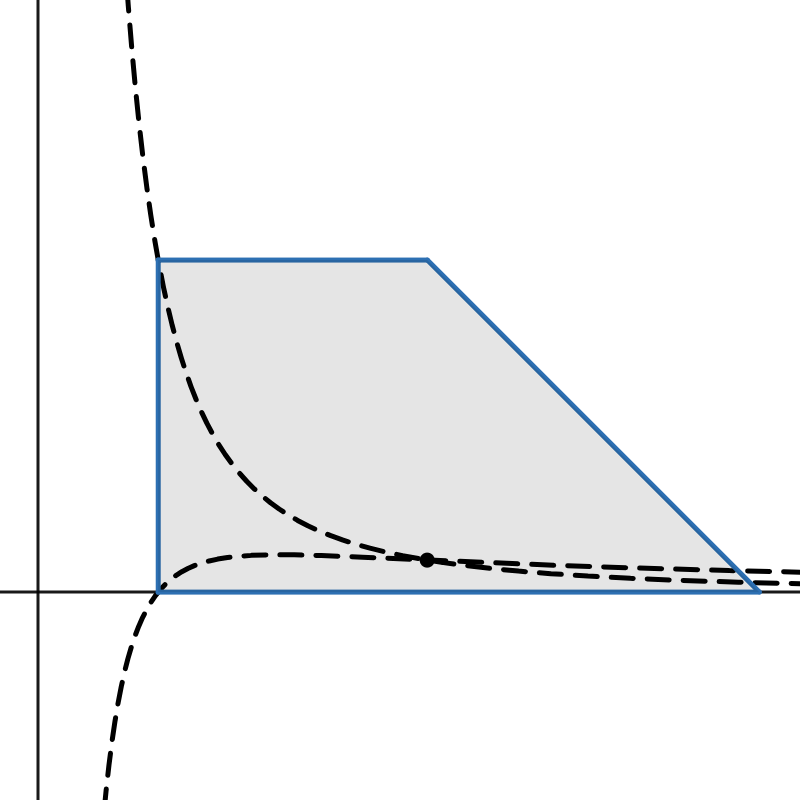
\includegraphics[width=0.4\textwidth]{figures/desmos-graph (24).png}
    \caption{The trapping region, plotted for $b = 2a$. The blue lines are the four lines decribed in the list: $x = a, y = 0, y = \frac{b}{a^2}$ and $y = a + b + \frac{b}{a^2} - x$. The dashed lines are the nullclines.}
\label{fig:part1a}
\end{figure}
As established, all derivatives in the normal direction to these lines lead into the area, meaning that it must be inlucded in some trapping region which is unescapable.
\subsection{Hopf bifurcation}
The system goes through a Hopf bifurcation when the eigenvalues are complex $D$ and reming complex as $\tau$ changes its sign. As we saw
\begin{equation}
    \tau = \frac{\eta}{\xi} - \xi^2
\end{equation}
will change its sign when
\begin{equation}
    \eta = \xi^3
\end{equation}
Or, in the original parameters:
\begin{equation}
    b - a = (a + b)^3
\end{equation}
Additionaly, Since $a,b > 0$, then $\xi = a + b > 0$, and thus $\Delta = \xi^2 > 0$. This means that when $\tau$ moves from positive to negative value, the discriminant will still have a complex part, making this a Hopf bifurcation.
\subsection{Criticallity of the Hopf bifurcation}
As we saw, this bifurcation happens withing a trapping region. From the Poincare-Bendixon theorem, as the point changes from a stable spiral to an unstable spiral, the flow away from the fixed point that still cannot leave the trapping region, must go to a limit cycle, and the Hopf bifurcation is defined as supercritical.
\subsection{The stability diagram}
Using the same data from section 1 (and Desmos), we can draw the stability diagram in the $a-b$:
\begin{figure}[H]
    \centering
    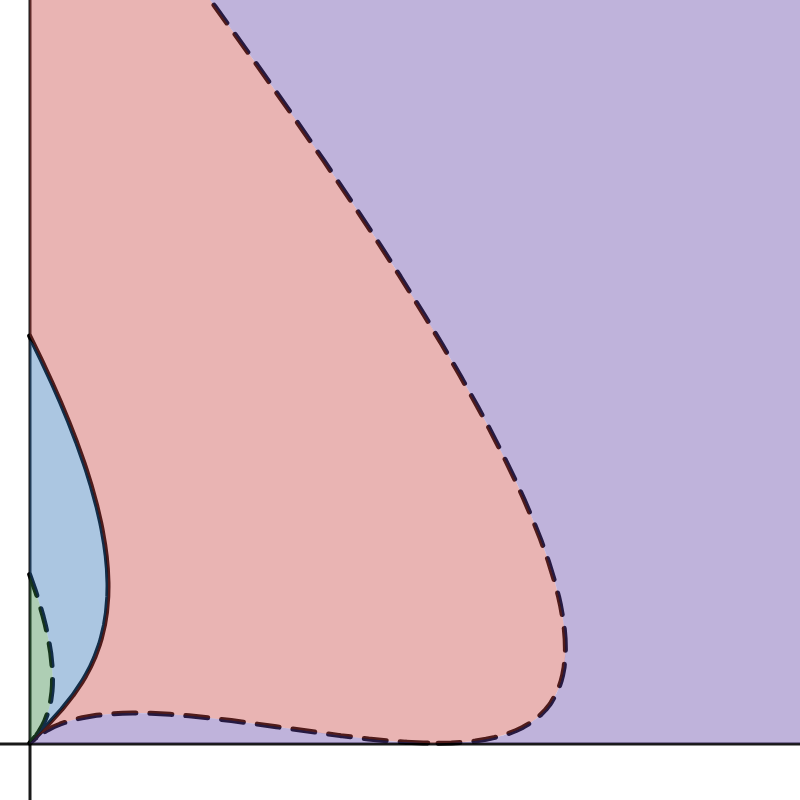
\includegraphics[width=0.5\textwidth]{figures/desmos-graph (26).png}
    \caption{The staibility diagagram in $a - b$ plain, with $a$ as the horizontal axis and $b$ as the vertical axis. The solid line describes the $\tau = 0$ line and the dashed lines describe the $D = 0$. This means that the green areas $\tau > 0, D > 0$} are the unstable nodes, the blue area $\tau > 0, D < 0$ is the unstable spiral with a limit cycle,
    the red area $\tau < 0, D < 0$ is the stable spiral fixed point, and the purple area $\tau < 0, D > 0$ is the stable node.
\end{figure}

\newpage
\section{Two-photon absorption}
We consider now the following 1D discrete time system:
\begin{equation}
    x_{n+1} = r + x_n - \alpha x_n^2
\end{equation}
\subsection{Fixed point}
Setting $x_{n+1} = x_n = x^*$ to find the fixed point:
\begin{equation}
    x^* = r + x^* - \alpha x^{*2}
\end{equation}
\begin{equation}
    0 = r - \alpha x^{*2}
\end{equation}
\begin{equation}
    x^* = \sqrt{\frac{r}{\alpha}}
\end{equation}
\subsection{Period doubling}
To find period doubling, we look for two points $x \ne y$ that map to eachother:
\begin{equation}
\begin{gathered}
    y = r + x - \alpha x^2
    \\
    x = r + y - \alpha y^2
\end{gathered}
\end{equation}
Moving things around
\begin{equation}
\begin{gathered}
    y - x + \alpha x^2 = r
    \\
    x - y + \alpha y^2 = r
\end{gathered}
\end{equation}
then adding and substracting them gives:
\begin{equation}
\begin{gathered}
    x^2 + y^2 = \frac{2r}{\alpha}
    \\
    x^2 - y^2 = \frac{2}{\alpha}(x - y) \rightarrow
    x + y = \frac{2}{\alpha}
\end{gathered}
\end{equation}
Plugging $y = \frac{2}{\alpha} - x$ into the first equation then gives:
\begin{equation}
    x^2 + \frac{4}{\alpha^2} - \frac{4x}{\alpha} + x^2 = \frac{2r}{\alpha}
\end{equation}
\begin{equation}
    x^2 - \frac{2}{\alpha}x + \frac{2 - r\alpha}{\alpha^2} = 0
\end{equation}
\begin{equation}
    x, y = \frac{1 \pm \sqrt{r\alpha - 1}}{\alpha}
\end{equation}
Which must be real, and so only have solutions for
\begin{equation}
    r \ge \frac{1}{\alpha}
\end{equation}
Another way to find the period doubling is to require that the derivative of the map will cross -1 from stable to unstable:
\begin{equation}
    m_1 = f'(x^*) < -1
\end{equation}
\begin{equation}
    f(x) = r + x - \alpha x^2 \rightarrow f'(x) = 1 - 2\alpha x
\end{equation}
\begin{equation}
    1 - 2\alpha x^* \le -1
\end{equation}
\begin{equation}
    2 - 2\alpha \sqrt{\frac{r}{\alpha}} \le 0
\end{equation}
\begin{equation}
    \alpha \sqrt{\frac{r}{\alpha}} \ge 1
\end{equation}
\begin{equation}
    r \ge \frac{1}{\alpha}
\end{equation}
So
\begin{equation}
    r_1 = \frac{1}{\alpha}
\end{equation}
\subsection{Stability of the Double period}
Using the same method (the second one), we can find the stability condition of the double period:
\begin{equation}
    \left|\left(f^2(x)\right)'\right| > 1
\end{equation}
\begin{equation}
\begin{gathered}
    m_2 = \left(f^2(x)\right)' = f'(x)f'(y) = \\ =
    (1 - 2\alpha x)(1 - 2\alpha y) = \\ =
    \left(1 - 2\left(1 + \sqrt{r\alpha - 1}\right)\right)\left(1 - 2\left(1 - \sqrt{r\alpha - 1}\right)\right) = \\ =
    1 - 2\left(1 + \sqrt{r\alpha - 1} + 1 - \sqrt{r\alpha - 1}\right) + 4\left(1 + \sqrt{r\alpha - 1}\right)\left(1 - \sqrt{r\alpha - 1}\right) = \\ =
    1 - 2 \cdot 2 + 4(1 - r\alpha + 1) = \\ =
    5 - 4 r\alpha
\end{gathered}
\end{equation}
Since $r, \alpha > 0$:
\begin{equation}
    \left|5 - 4 r\alpha\right| > 1 \rightarrow 5 - 4 r\alpha < -1
\end{equation}
\begin{equation}
    r > \frac{1.5}{\alpha}
\end{equation}
\begin{equation}
    r_2 = \frac{1.5}{\alpha}
\end{equation}
\subsection{Variable change}
We are looking for a new variable such that:
\begin{equation}
    y_{n+1} = 1 - \mu y_n^2
\end{equation}
Assuming, based on the similarity of forms, that the trasnformation is a linear map:
\begin{equation}
    y_n = a x_n + b
\end{equation}
Plugging this in:
\begin{equation}
    a x_{n+1} + b = 1 - \mu (a x_n + b)^2
\end{equation}
\begin{equation}
    x_{n+1} = \frac{1 - b}{a} - \mu a x_n^2 - 2\mu bx_n - \frac{\mu b^2}{a}
\end{equation}
\begin{equation}
    x_{n+1} = \frac{1 - b - \mu b^2}{a} - 2\mu bx_n - \mu a x_n^2
\end{equation}
For this to be the same as the original system, we require:
\begin{equation}
    \frac{1 - b - \mu b^2}{a} = r
    \qquad
    - 2\mu b = 1
    \qquad
    \mu a = \alpha
\end{equation}
The last two conditions give:
\begin{equation}
    b = -\frac{1}{2\mu}
    \qquad
    a = \frac{\alpha}{\mu}
\end{equation}
Plugging this into the first equation gives:
\begin{equation}
    \frac{1 + \frac{1}{2\mu} - \mu \frac{1}{4\mu^2}}{\frac{\alpha}{\mu}} = r
\end{equation}
\begin{equation}
    \frac{4 \mu + 1}{4 \alpha} = r
\end{equation}
\begin{equation}
    \mu = \frac{4 \alpha r - 1}{4}
\end{equation}
In summary:
\begin{equation}
    y_n = 2\frac{2 \alpha x_n - 1}{4 \alpha r - 1}
    \qquad
    \mu = \frac{4 \alpha r - 1}{4}
\end{equation}
\subsection{First three period doubling}
Isolating $r$ from the $\mu(r)$ relation:
\begin{equation}
    r = \frac{4\mu + 1}{4\alpha}
\end{equation}
Which gives:
\begin{equation}
    \mu_1 = 1 \rightarrow r_1 = \frac{5}{4\alpha}
\end{equation}
\begin{equation}
    \mu_2 = \frac{3}{2} \rightarrow r_2 = \frac{7}{4\alpha}
\end{equation}
\begin{equation}
    \mu_3 = 1.543 \rightarrow r_3 = \frac{1.793}{\alpha}
\end{equation}
\subsection{The Lyapunov exponent}
The Lyapunov exponent of a orbit starting from $x_0$:
\begin{equation}
    \Lambda (x_0) = \lim_{n \rightarrow \infty} \frac{1}{n} \sum_{i=0}^{n-1} \ln\left|f'(x_i)\right|
\end{equation}
For a periodic k-cycle, this is simplified to
\begin{equation}
    \Lambda_k = \frac{1}{k} \sum_{i=0}^{n-1} \ln\left|f'(x_i)\right| = \frac{1}{k} \ln\left|\prod_{i=0}^{n-1} f'(x_i)\right| = \frac{1}{k} \ln\left|m_k\right|
\end{equation}
For $k = 1, 2$, this gives:
\begin{equation}
    \Lambda_1(r) = \ln|1 - 2\sqrt{\alpha r}|
    \qquad
    \Lambda_2(r) = \frac{1}{2}\ln|5 - 4\alpha r|
\end{equation}
For $r_0 = 0$, we get the start of the 1-cycle (fixed point):
\begin{equation}
    \Lambda_1(r_0) = 0
\end{equation}
For $r_1 = \frac{1}{\alpha}$, we get the end fo the 1-cycle and teh start of the 2-cycle
\begin{equation}
    \Lambda_1(r_1) = \Lambda_2(r_1) = 0
\end{equation}
For $r_2 = \frac{1.5}{\alpha}$, we get the end of the 2-cycle
\begin{equation}
    \Lambda_2(r_2) = 0
\end{equation}
\end{document}